\section{Passwortcracker}
\subsection{Passwortcrackers HEL}
\paragraph{Gegebener Hinweis:} „Lang lebe die Anarchie...die Kapitalisten müssen sterben...9 Zeichen...ein Wort mit 7 Kleinbuchstaben, welches man sich gut merken kann, dann eine Zahl und ein Sonderzeichen. Das sollte für die Imperialisten reichen...“

Daraus ergibt sich die Passwort-Komplexität:
$$
[a-zäöüß]^7[0-9][\text{34 Sonderzeichen}]
\Rightarrow 
n = 30^7 \cdot 10^1 \cdot 34^1 
= 7,4358 \cdot 10^{12}
\approx 2^{43}                                                                                                                                   
$$
Es handelt sich hier um ein 43-Bit Problem im Worst Case, 42-Bit im Average Case. Der Passwortcracker kann $2^{42}$ Passwörter pro Sekunde raten. Daher:
$$
t(k)=
\frac{
2^{k} \text{ Passwörter}
}{
2^{47} \frac{Passwörter}{Sekunde}
}
$$
Im Worst Case, $k=43$:
$$
t(43)
= \frac{
2^{43} \text{ Passwörter}
}{
2^{47} \frac{Passwörter}{Sekunde}
}
= 2^{-4} \text{ Sekunde(n)}
\rightarrow 0,0625 \text{ Sekunden}
$$ Im Avarage-Case, $k=42$:
$$
t(42)
= \frac{
2^{42} \text{ Passwörter}
}{
2^{47} \frac{Passwörter}{Sekunde}
}
= 2^{-5} \text{ Sekunde(n)}
\rightarrow 0,03125 \text{ Sekunde}
$$
Zusätzlich kann der Angriff mit einem Dictionary-Angriff kombiniert werden. Dazu wird eine Dictionary Datei gefiltert, sodass nur die Wörter mit 7 Buchstaben verwendet werden. Diese müssen lower case gemacht werden. Daraus ergibt sich in unserem Beispiel eine Wort-Komplexität von
$$
25.751 \text{ (Zeilen)} \cdot  [0-9][\text{34 Sonderzeichen}]
\Rightarrow
n = 25.751 \cdot 10^1 \cdot 34^1
= 8.755.340
\approx 2^{23}                                                                                                                                   
$$
Daraus ergibt sich eine Rechenzeit von:
$$
t(23)
= \frac{
2^{23} \text{ Passwörter}
}{
2^{47} \frac{Passwörter}{Sekunde}
}
= 2^{-24} \text{ Sekunde(n)}
\rightarrow 0,00000006 \text{ Sekunden}
$$ \subsection{Anderes Passwort}
$$
[\textbf{A-Za-zöäü0123456789!?}]^{12} \Rightarrow 67^{12} \approx 2^{73}
$$
HEL bräuchte daher im Worst Case $
t(73)= 2^{31} \text{ Sekunden} = 2147483648 \text{ Sekunden}
$. Das entspricht ungefähr 68 Jahren, im Average Case 34 Jahre.


\subsection{Passwort Bildungsgesetz}

Es gilt, zwischen Passwörtern zu unterscheiden, die man sich merken muss und bei denen ein Passwortmanager verwendet wird. Von Passwortmanagern verwaltete Passwörter sollten möglichst echt-zufällig generiert werden. Bei Merkpasswörtern kann ein Trick verwendet werden, der es erleichtert, sich das Passwort zu merken:

Ein Text wird auswendig gelernt (z.B.  Gedicht / Song / sonstiges). Anfangsbuchstaben und Sonderzeichen werden übernommen. Gegebenenfalls werden noch weitere Sonderzeichen hinzufügen bzw. aus Buchstaben/Wörtern interpretieren. Somit kann sich ein scheinbar zufällig generiertes Passwort gemerkt werden. 

Grundsätzlich ist eine Entropie von 256 Bit optimal. Ausgehend von 95 Druckbaren ASCII-Zeichen:
$$
95^x = 2^{256} \Leftrightarrow x = log_{95}(2^{256}) = 38,965848759 \approx 39 \rightarrow 39 \text{ Zeichen}
$$
Ein Passwort sollte also aus 39 der 95 ASCII-Zeichen bestehen. Die Komplexität wird noch größer, sollten Unicode-Zeichen verwendet werden, die nicht von ASCII abgedeckt werden.

\subsection{Cracken des Truecryptcontainer mit Hashtopolis}
Folgend galt es mithilfe von Hashtopolis und dem damit Zusammenhängenden Passwortcracker der HS-Emden-Leer, den Truecryptcontainer für das LKA Niedersachsen zu öffnen.\\
Wir haben gestartet und uns unter der 10.10.10.20 bei Hashtopolis einzuloggen.
\begin{figure}[h]
\raggedright
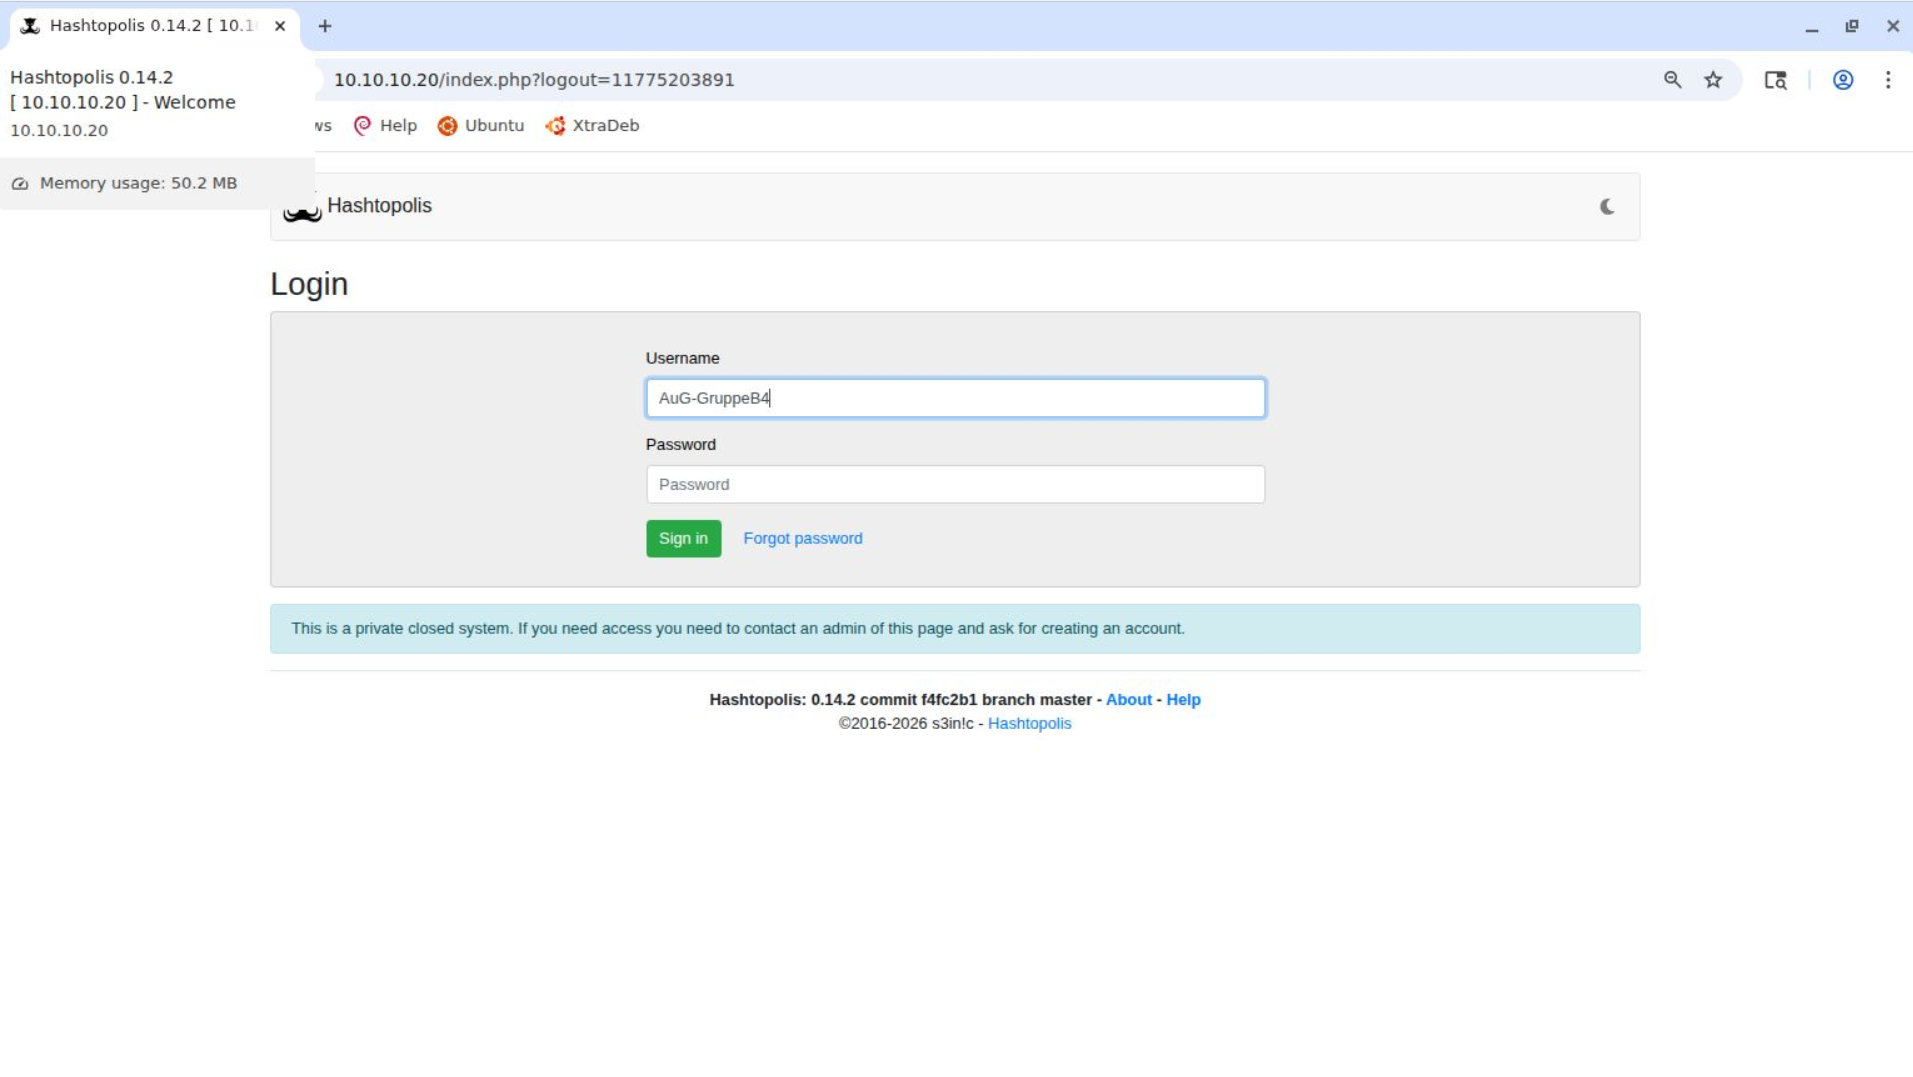
\includegraphics[width=0.7\textwidth]{img/PW-loginHashtopolis.png}
\end{figure}
\\
Anschließend, wie der Anleitung zu entnehmen, haben wir den Truecrypt Container hochgeladen vom Type: TrueCrypt 5.0+ PBKDF2-HMAC-RipeMD160 + AES/Serpent/Twofish als neue Hashliste.
\newpage
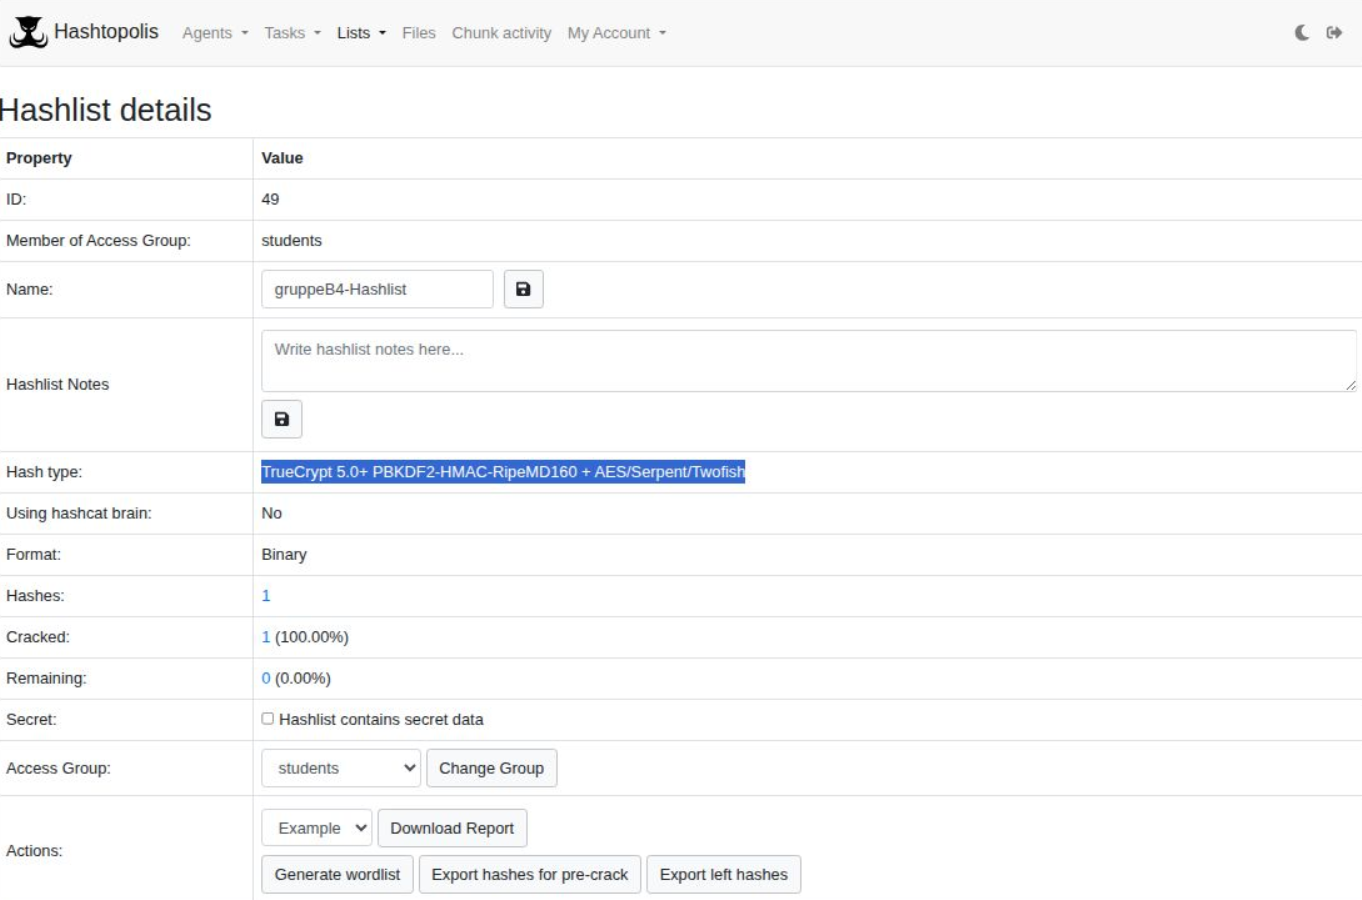
\includegraphics[width=0.7\textwidth]{img/Screenshot 2026-04-03 101952.png}
\\
Damit haben wir dann eine Task erstellt, welche wir im Hashcat-Format Anweisung zum Cracken des PW gegeben haben.\\
Nämlich wie unsere Geheime abgefangene Nachricht verraten hat suchen wir ein Passwort, welches aus 7 Kleinbuchstaben sowie folgend 1 Zahl und ein Sonderzeichen hat.\\
Dazu haben wir folgenden Befehl aufgestellt:
\begin{verbatim}
-a 6 -m 6211 #HL# 7char-words-lc-utf8-cc24.dic ?d?s
\end{verbatim}
-a 6 steht dabei für den Hybrid Modus - Wörterbuch und Maske verwenden , -m 6211 steht für unseren Hashtype.\\
\#HL\# unserer Liste die wir angelegt haben mit dem Truecryptcontainer und dann die Wörterliste welche alle 7 langen Wörter beinhaltet. Zusätzlich passend zum Modus dann zusätzlich die Maske ?d?s.
\begin{verbatim}
    ?d = 0123456789 
    ?s = !"#$%&'()*+,-./:;<=>?@[\]^_`{|}~
    Siehe auch HashcatCheatSheet
\end{verbatim}
Task ist erstellt, dann muss ein Agent zugewiesen werden und die Suche nach dem Passwort beginnt.
Wir hatten Erfolg und das Passwort konnte gefunden werden\\
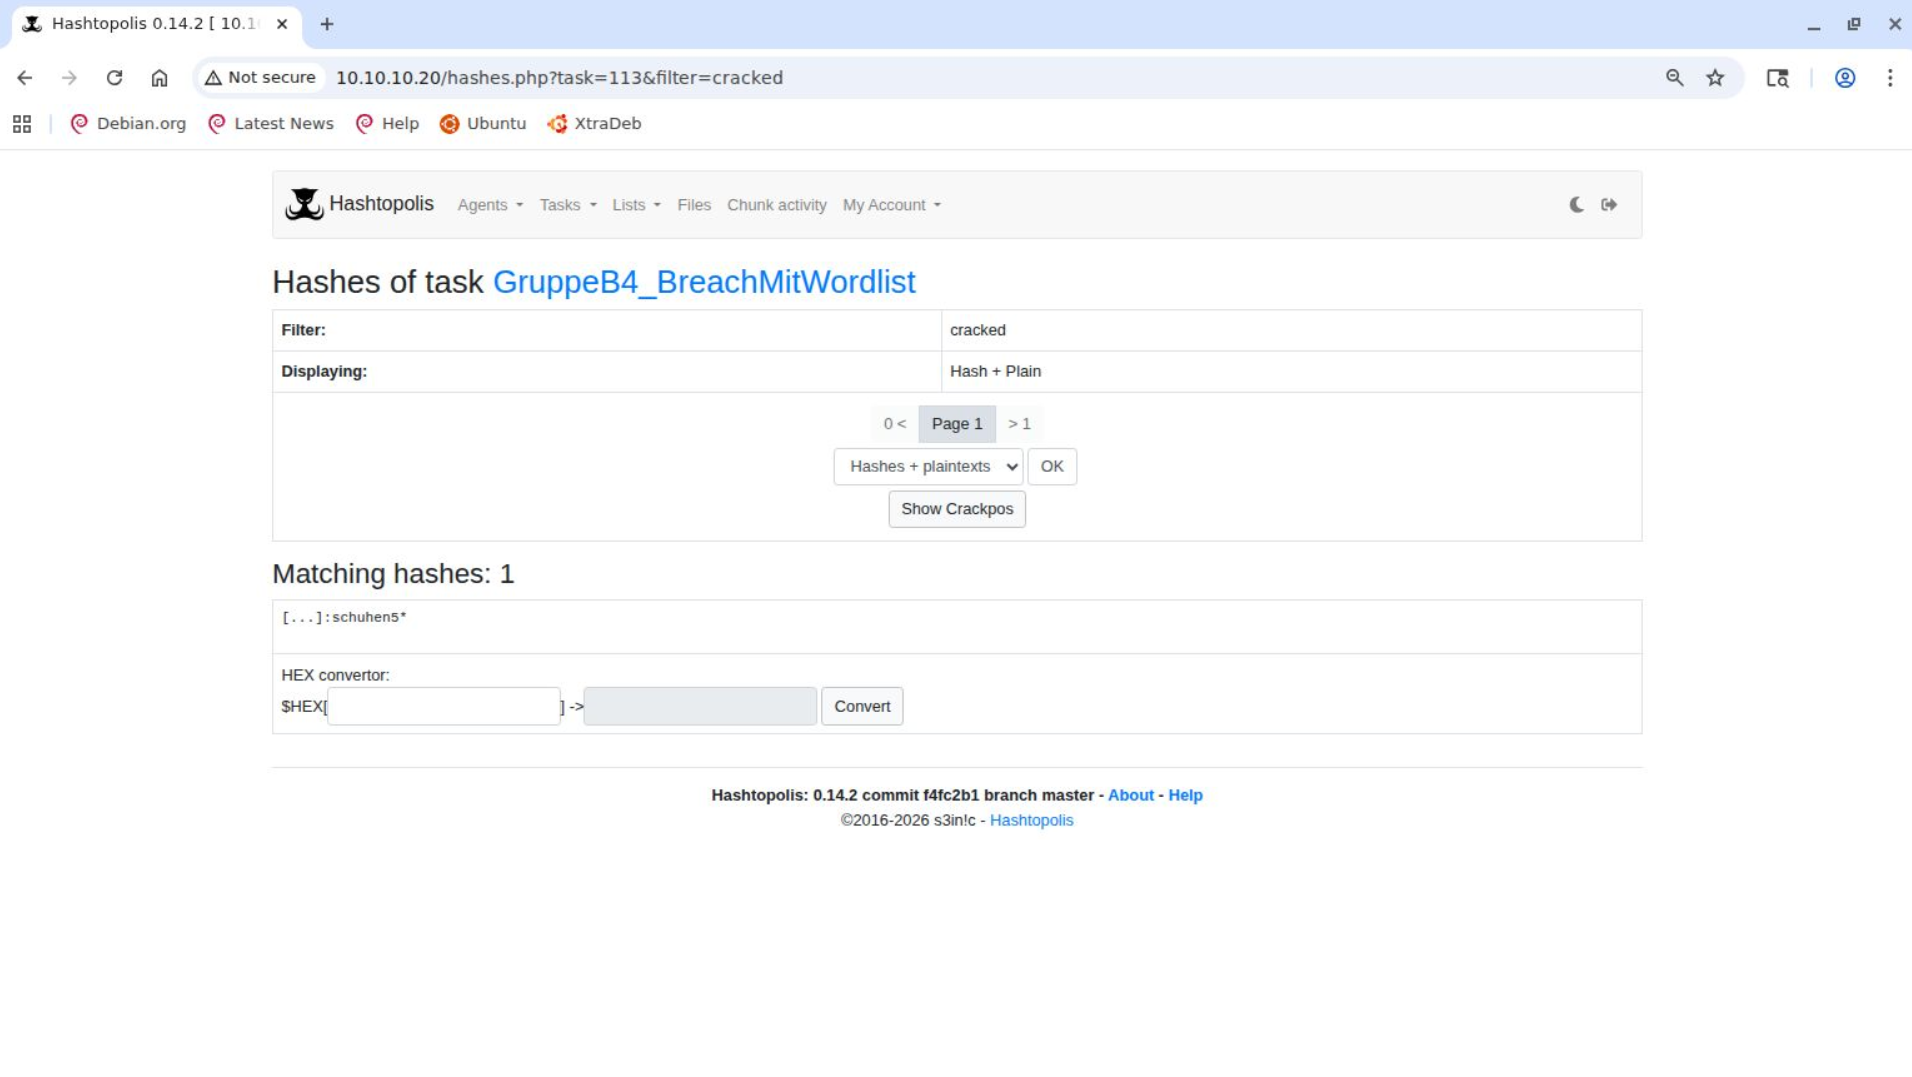
\includegraphics[width=0.7\textwidth]{img/PWFound.png}\\[1cm]
Nun mit dem gefunden Passwort \texttt{Schuhen5*} den TrueCrypt-Container entschlüsseln und öffnen. Dadurch wurde ein Speichermedium unlocked der die Datei enthalten hat, die wir dann auslesen konnten.\\
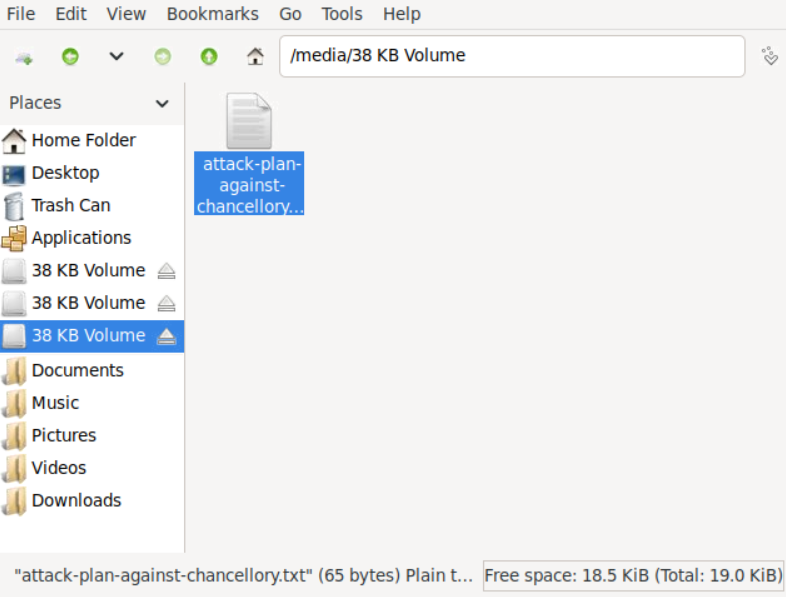
\includegraphics[width=0.7\textwidth]{img/PWContainerCracked.png}
